\chapter{Umsetzung}
    Die Entwicklung der Platzierungssoftware erfolgte in Java-SE 11.
    Der grobe Ablauf des Programmes besteht darin, die Netzliste sowie die fixierten Pads
    einzulesen und daraus ein Graphen zu erstellen.
    Dadurch, dass es im Praktikum nur eine relevante FPGA-Architektur zu betrachten gab,
    wurde vom Einlesen der *.arch Datei abgesehen und die benötigten Parameter wurden über
    Konstanten direkt im Programmcode abgelegt. Wurde der Graph erfolgreich erstellt wird
    eine Initialplatzierung vorgenommen. 
    Kapitel (\ref{sec:init}) beschreibt hierbei die vom Grundalgorithmus abweichende Vorgehensweise
    um die Ergebnisse der Platzierung zu Optimieren. Nach Abschluss der Initialplatzierung
    beginnt die eigentliche Optimierung der Platzierung. Kapitel (\ref{sec:algo}) geht dabei auf die genauen
    Einzelheiten des Algorithmus ein.
    Nach Abschluss des Algorithmus wird aus der aktuellen Platzierung die
    Platzierungsdatei erstellt und ausgegeben.


    \begin{figure}[H]
        \centering
        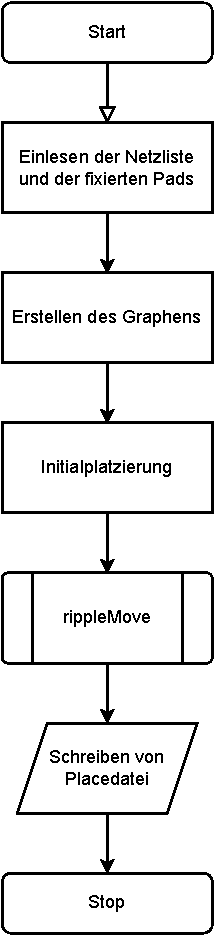
\includegraphics[scale=0.75]{img/Programm-flowchart.pdf}
        \caption{Programmablaufplan}
        \label{fig:program-flowchart}
    \end{figure}

        

    \section{Programmstruktur}

        Abbildung (\ref{fig:uml}) zeigt das UML-Diagramm des Programmes.
        Die Hauptlogik des Programmes befindet sich in der FPGA-Klasse,
        die zuständig für die Platzierung der Logikblöcke ist.
        Als wichtigste Komponente gilt der Graph, der durch die die eingelesenen Blöcke sowie die
        fixierten Pads erstellt wird und der FPGA-Instanz beim Instanziieren übergeben wird.
        Über die Methoden \textit{initPlace} oder \textit{randomPlace} wird eine Initialplatzierung vorgenommen.
        Des weiteren wird über die Methode \textit{rippleMove} die eigentliche Optimierung der Platzierung
        vorgenommen.
        \begin{figure}[H]
            \centering
            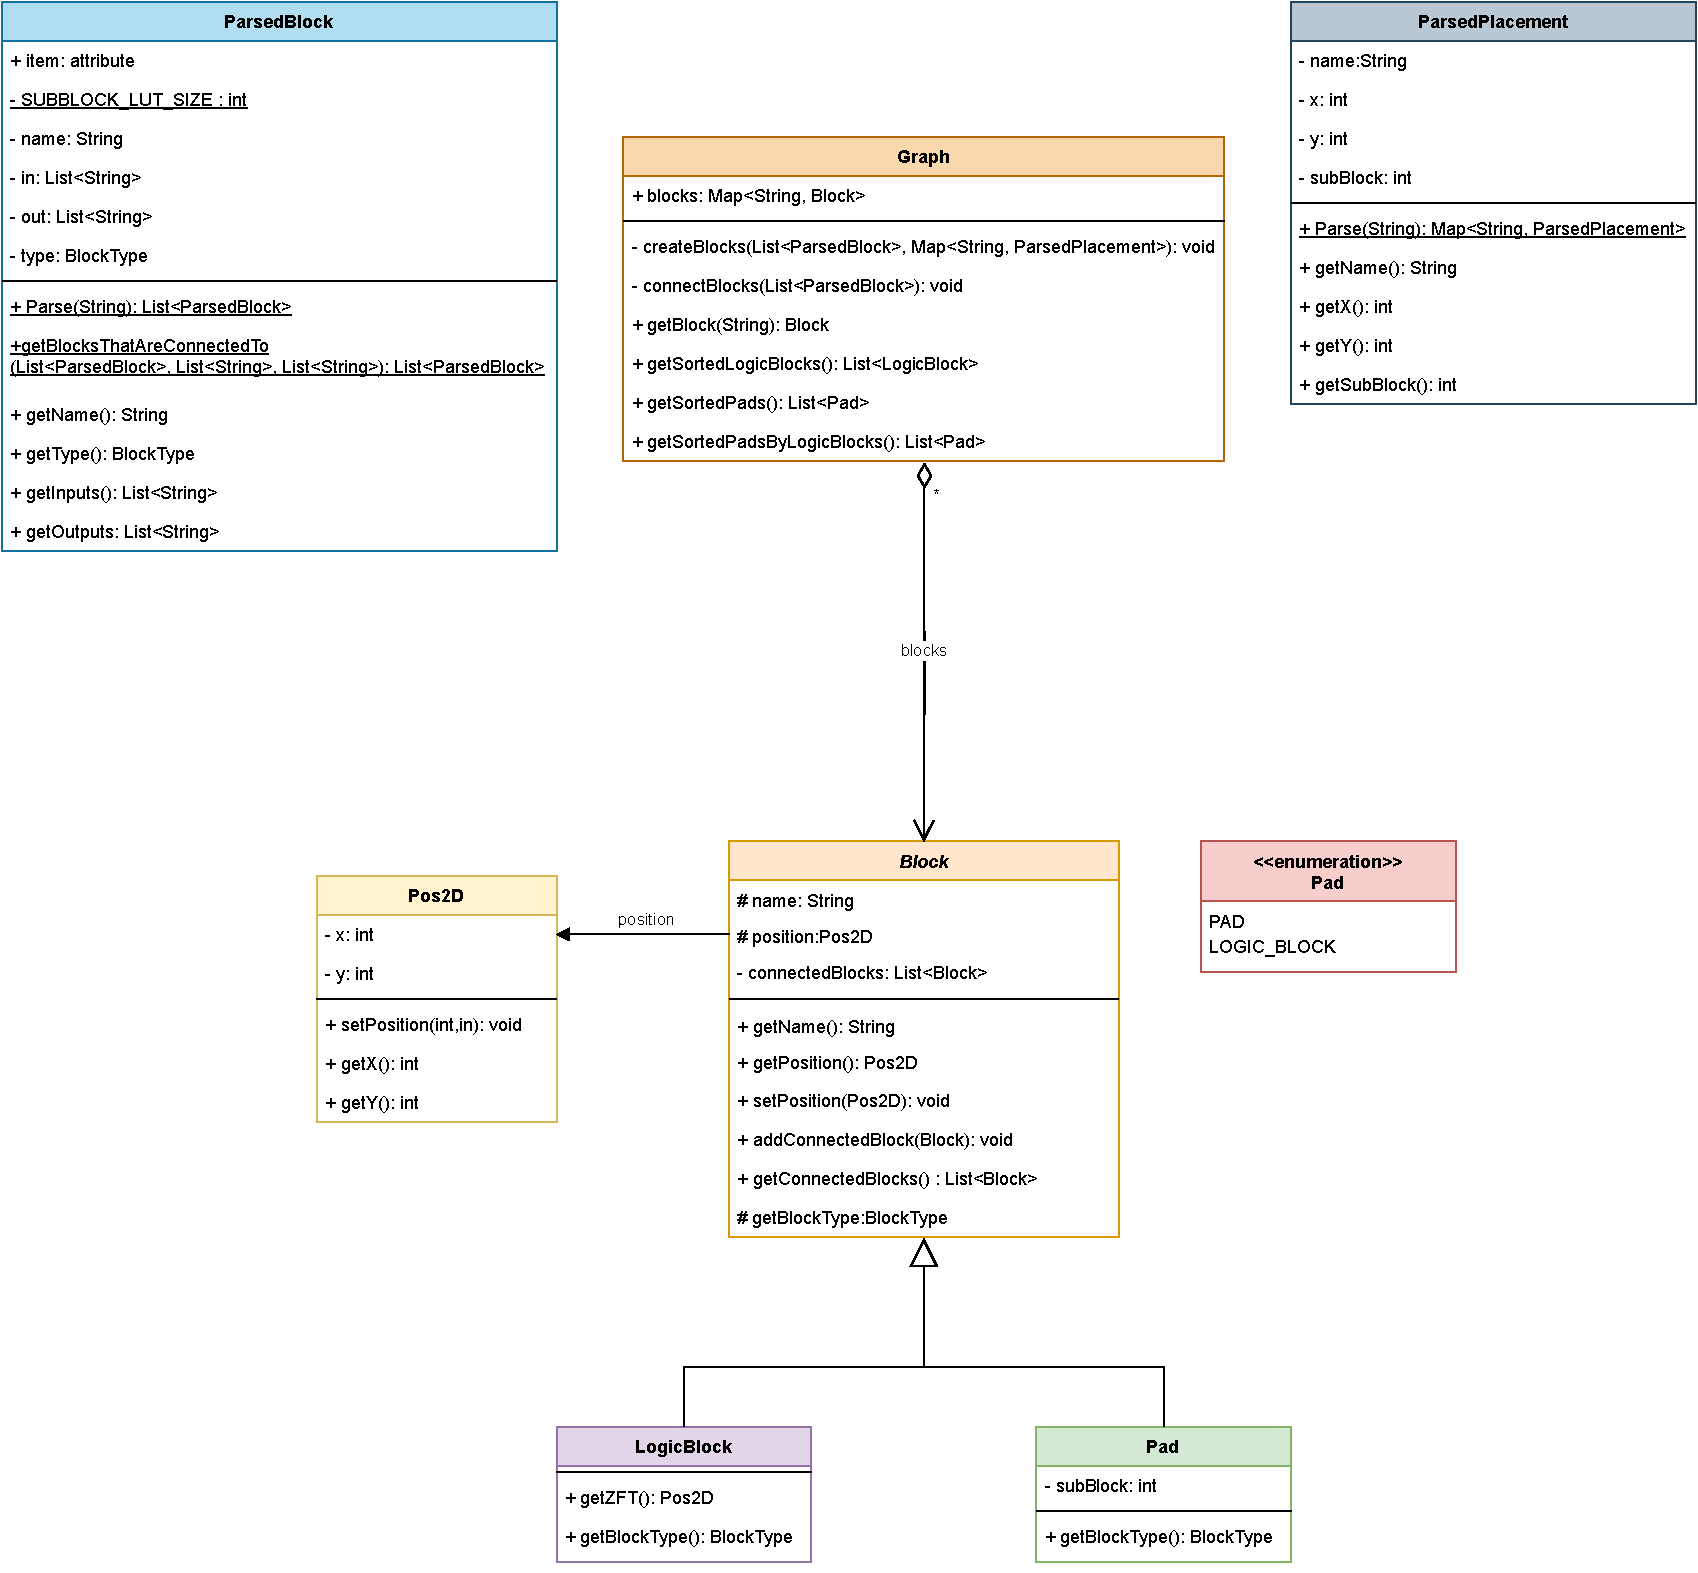
\includegraphics[width=\textwidth]{img/UML.pdf}
            \caption{UML Diagramm}
            \label{fig:uml}
        \end{figure}

    
        
    \section{Initialplatzierung}\label{sec:init}
     

    \section{Algorithmusablaufplan}\label{sec:algo}
        Zunächst werden die Logikblöcke absteigend nach ihrem Verbindungsgrad sortiert.
        Das heißt, dass Blöcke mit mehr Verbindungen weiter vorne in der Liste stehen.
        Dies hat den Vorteil, dass diese Blöcke besser platziert werden können.
        Als Nächstes werden die Blöcke iterativ durchlaufen und für jeden Block die ZFT-Position ermittelt.
        \\
        Ist die Zielposition schon fixiert, das heißt, dass ein anderer Block in
        diesem Iterationsschritt auf die Zielposition gesetzt wurde, wird
        Zunächst der rippleIteration Zähler erhöht und verglichen,
        ob dieser größer bzw. gleich der \textit{maxRippleIteration} Variable ist.
        Ist dies der Fall, wird in der Nähe der Zielposition die nächste freie
        Zelle gesucht und der aktuelle Block auf diese Position gesetzt.
        Des Weiteren wird die maxIteration Zählervariable dekrementiert,
        alle Fixierungen werden gelöst und der Algorithmus beginnt eine neue Iteration. 
        \\
        In dem Fall, dass die \textit{maxRippleIterations} nicht überschritten wurde,
        wird die beste Position in der Nähe der Zielposition gesucht.
        Dabei werden alle anliegenden Positionen betrachtet und die Position ausgewählt,
        an dem der aktuelle Block der niedrigsten Kraft ausgesetzt ist.
        Die neue Zielposition wird daraufhin wieder auf die drei Hauptbedingungen geprüft.
        \\
        Ist die Zielposition nicht fixiert und der Block ist schon auf seiner Zielposition
        werden die \textit{rippleIteration} Variable zurückgesetzt und die Zielposition fixiert.
        \\
        Ist die Zielposition jedoch belegt und nicht fixiert, wird der aktuelle Block
        auf die Zielposition gesetzt, die Position fixiert, der \textit{rippleIteration} Zähler zurückgesetzt
        und der verdrängte Block wird auf den aktuellen Block gesetzt.
        Als Nächstes startet der Algorithmus an der Stelle, an dem die ZFT-Position für den
        aktuellen Block (verdrängter Block) berechnet wird.
        Als letzte Bedingung kann die Zielposition unbelegt sein.
        Ist dies der Fall wird der aktuelle Block auf die Zielposition gesetzt,
        die Position fixiert und der \textit{rippleIteration} Zähler zurück gesetzt.
        Ist der \textit{maxIterations} auf Null dekrementiert worden wird der Algorithmus beendet.

        \begin{figure}[H]
            \centering
            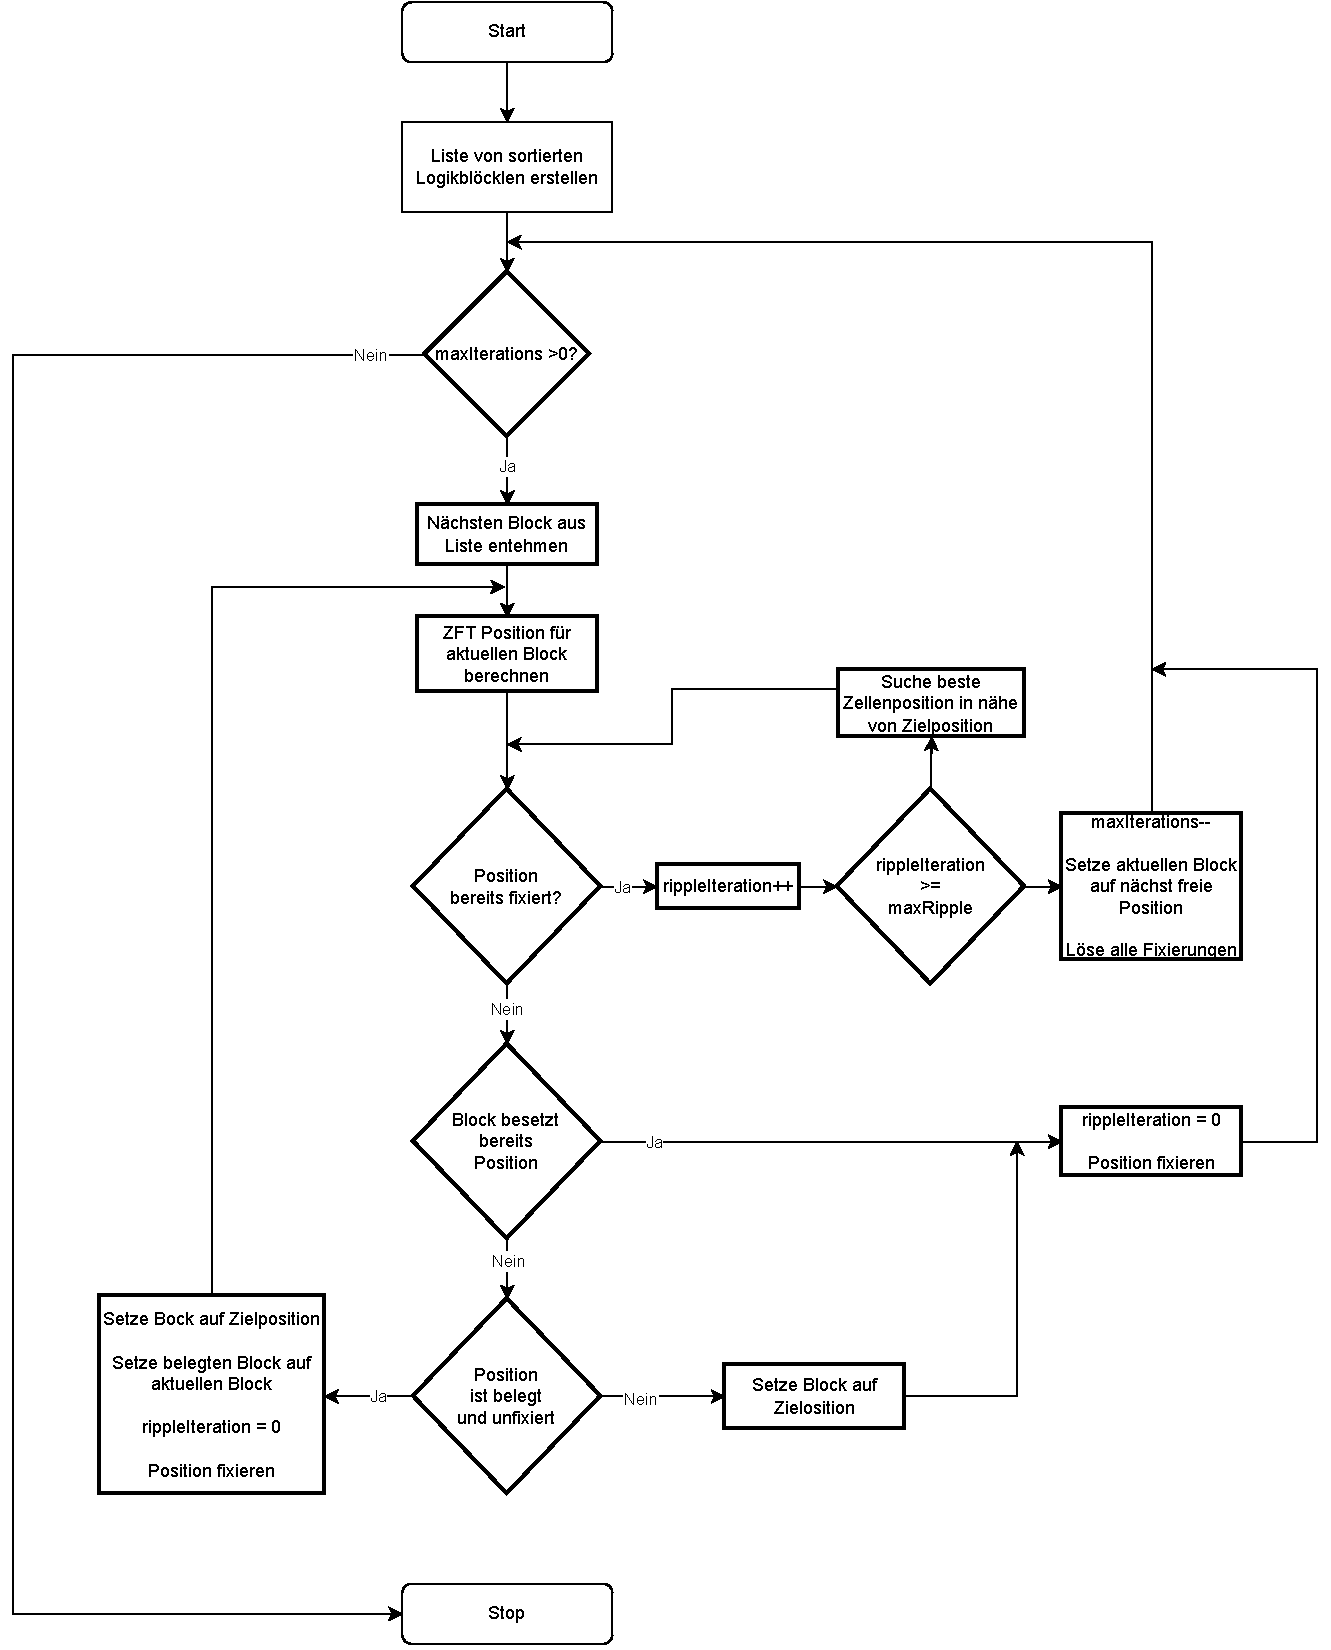
\includegraphics[width=\textwidth]{img/flowchart.pdf}
            \caption{Algorithmusablaufplan}
            \label{fig:algo-flowchart}
        \end{figure}
